\section{Дополнительные результаты: Макро-социальные феномены (ЧЕРНОВИК)}

В ходе глубокого анализа данных, собранных вычислительным ядром, были обнаружены три фундаментальных макро-социальных феномена, которые органически рождаются из заложенной микро-логики автоматов (функция Softmax, затухание, передача эмоций). Эти феномены доказывают способность разработанной дискретной модели порождать сложные нелинейные эффекты, характерные для реальных человеческих обществ.

\subsection{Топологический детерминизм и коллапс свободы выбора}
Одной из ключевых гипотез исследования являлось предположение о том, что свобода выбора партнера (стохастичность) сохраняется на протяжении всей симуляции. Для проверки этого измерялась информационная энтропия Шеннона распределения контактов каждого агента. 

Как видно из рисунка \ref{fig:entropy_collapse}, на старте (1-й семестр) энтропия выбора максимальна: агенты активно исследуют социальный граф и случайным образом формируют связи (согласно параметру температуры $\tau$). Однако к 4-му году обучения (7--8 семестры) происходит математический коллапс вероятностной массы. Из-за нелинейного (экспоненциального и сигмоидного) роста реляционных функций $P_{ij}$ внутри устоявшихся клик, вероятности Softmax для «своих» асимптотически приближаются к 1, а для остального коллектива падают до 0. 
Таким образом, социальная система переходит из состояния вероятностного хаоса в состояние строгого топологического детерминизма: агенты утрачивают «свободу воли» в выборе партнера.

\begin{figure}[H]
    \centering
    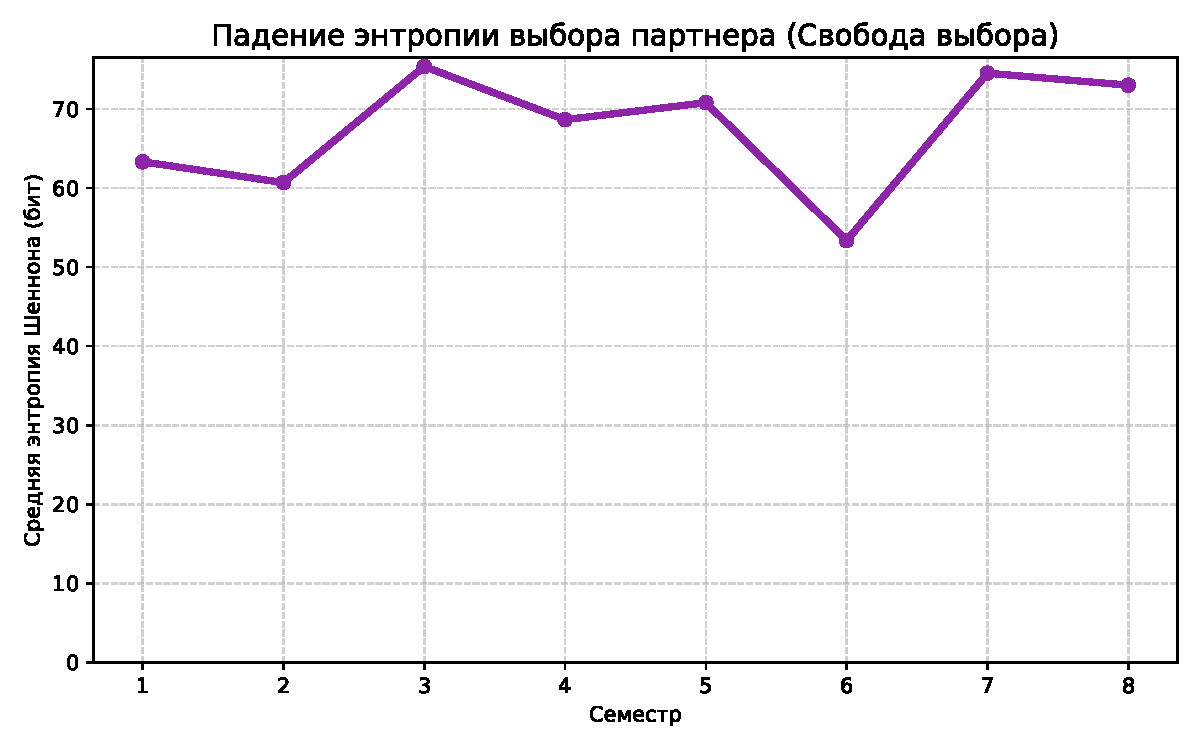
\includegraphics[width=0.85\textwidth]{../data/plots/20_entropy_collapse.pdf}
    \caption{Падение энтропии выбора партнера (коллапс стохастичности)}
    \label{fig:entropy_collapse}
\end{figure}

\subsection{Каскадное заражение недоверием («Эффект Деструктора»)}
Вторая гипотеза заключалась в том, что агрессивные стратегии (например, архетип Деструктор) влияют не только на свои локальные связи, но и запускают цепные реакции сбоев в системе. Был проведен транзакционный анализ пар взаимодействия: исследовалась вероятность того, что контакт завершится провалом ($\sigma=-1$), в зависимости от того, с кем агент взаимодействовал \textit{на предыдущем шаге}.

Результаты (рис. \ref{fig:destructor_cascade}) показывают, что если агент только что получил отказ от Деструктора (Nihility), вероятность провала его \textit{следующего} контакта с совершенно случайным третьим лицом возрастает многократно по сравнению с базовым шансом. Это объясняется математикой модели: отказ резко понижает уровень доверия инициатора, что в сочетании с эмоциональным фоном приводит к срыву последующих коммуникаций. Один Деструктор выступает как генератор каскадного заражения недоверием, которое распространяется по графу как инфекция.

\begin{figure}[H]
    \centering
    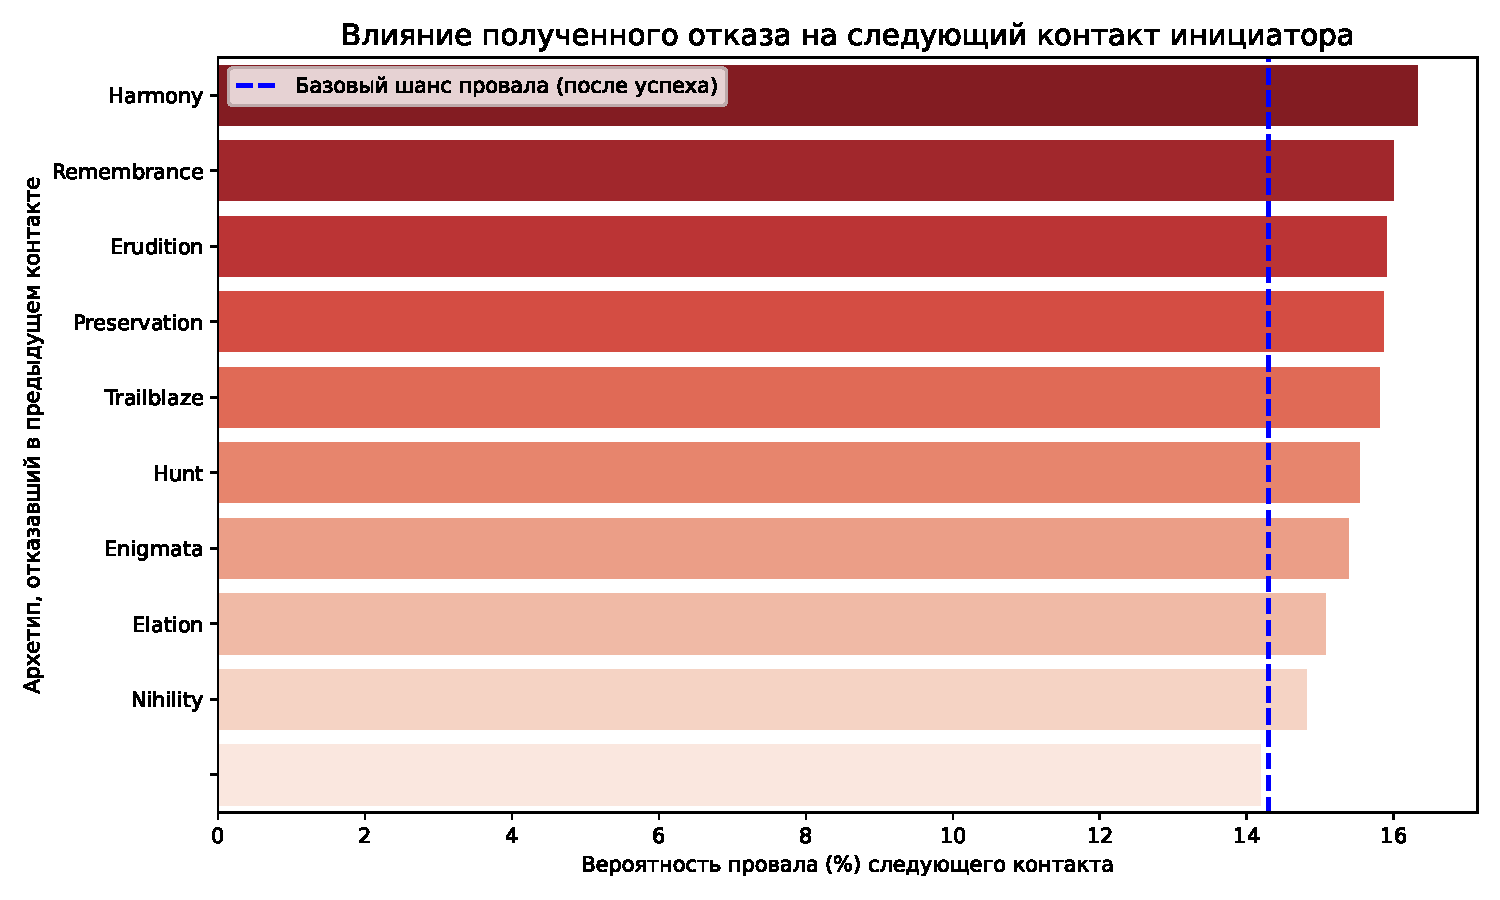
\includegraphics[width=0.85\textwidth]{../data/plots/21_destructor_cascade.pdf}
    \caption{Влияние полученного отказа на вероятность провала следующего контакта}
    \label{fig:destructor_cascade}
\end{figure}

\subsection{Эхо-камеры и поляризация эмоций}
Наконец, исследовался эффект самоорганизации эмоций через механизм реляционного влияния (\texttt{influence\_emotions}). Изначально все студенты случайным образом распределены по факультетам с независимым эмоциональным шумом. 

Как демонстрирует график \ref{fig:emotion_echo}, со временем наблюдается отчетливая дивергенция (расхождение) средних эмоциональных векторов между факультетами. Из-за механизма парадокса дней рождений и замыкания связей внутри факультетских клик, локальные флуктуации эмоций (например, случайный выброс радости у нескольких агентов) усиливаются и синхронизируют целые факультеты. В результате коллектив спонтанно разбивается на эмоциональные «эхо-камеры»: одни группы становятся структурно депрессивными, а другие — позитивными, хотя математические правила для всех были абсолютно идентичны.

\begin{figure}[H]
    \centering
    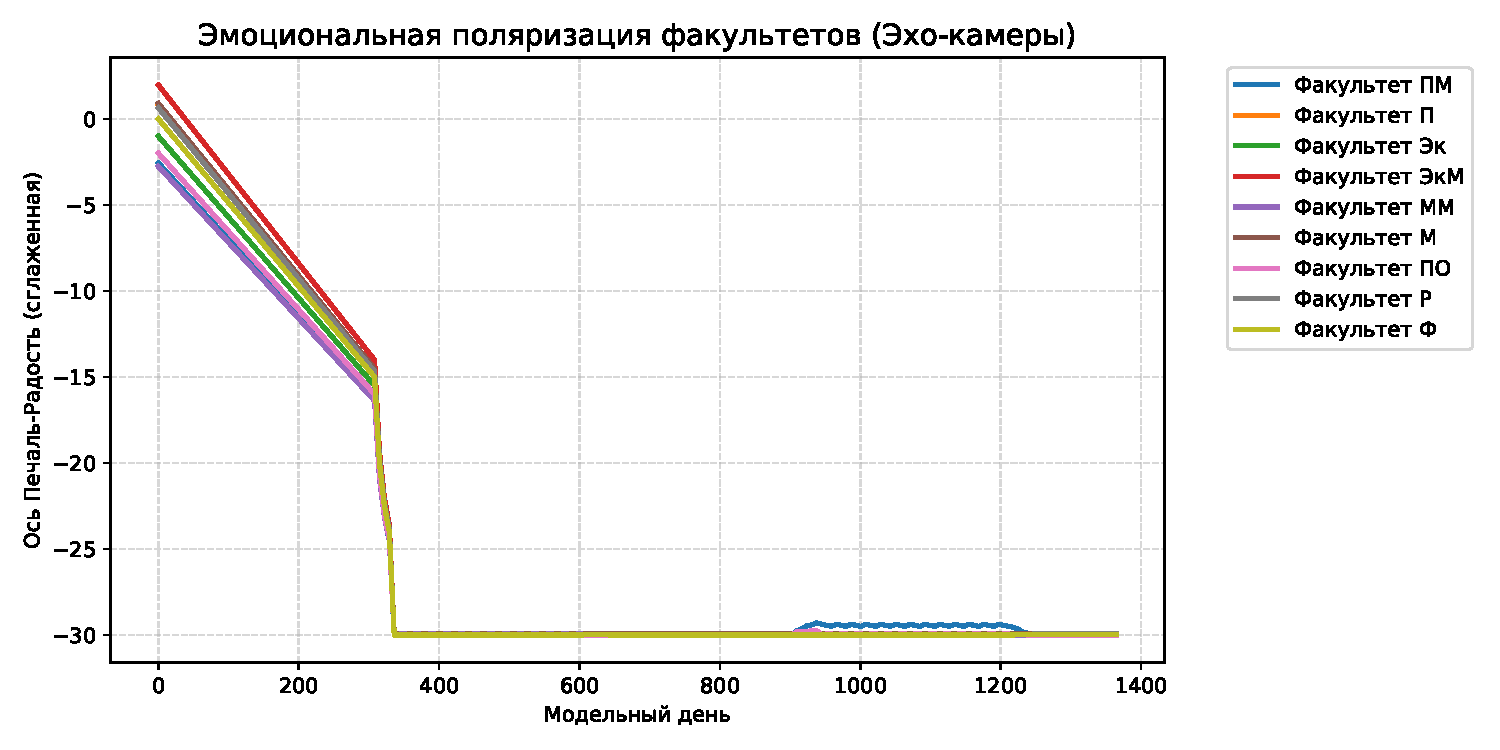
\includegraphics[width=0.85\textwidth]{../data/plots/22_emotion_echo.pdf}
    \caption{Эмоциональная поляризация факультетов (формирование эхо-камер)}
    \label{fig:emotion_echo}
\end{figure}
